\documentclass[../main/main.tex]{subfiles}

\raggedbottom

\makeatletter
\renewcommand{\@chapapp}{\'Electrocin\'etique -- chapitre}
\makeatother

\toggletrue{student}

\begin{document}
\setcounter{chapter}{6}

\chapter{Filtrage lin\'eaire}

\section{Signaux périodiques}
\subsection{Période}

\subsection{Moyenne}
\begin{center}
    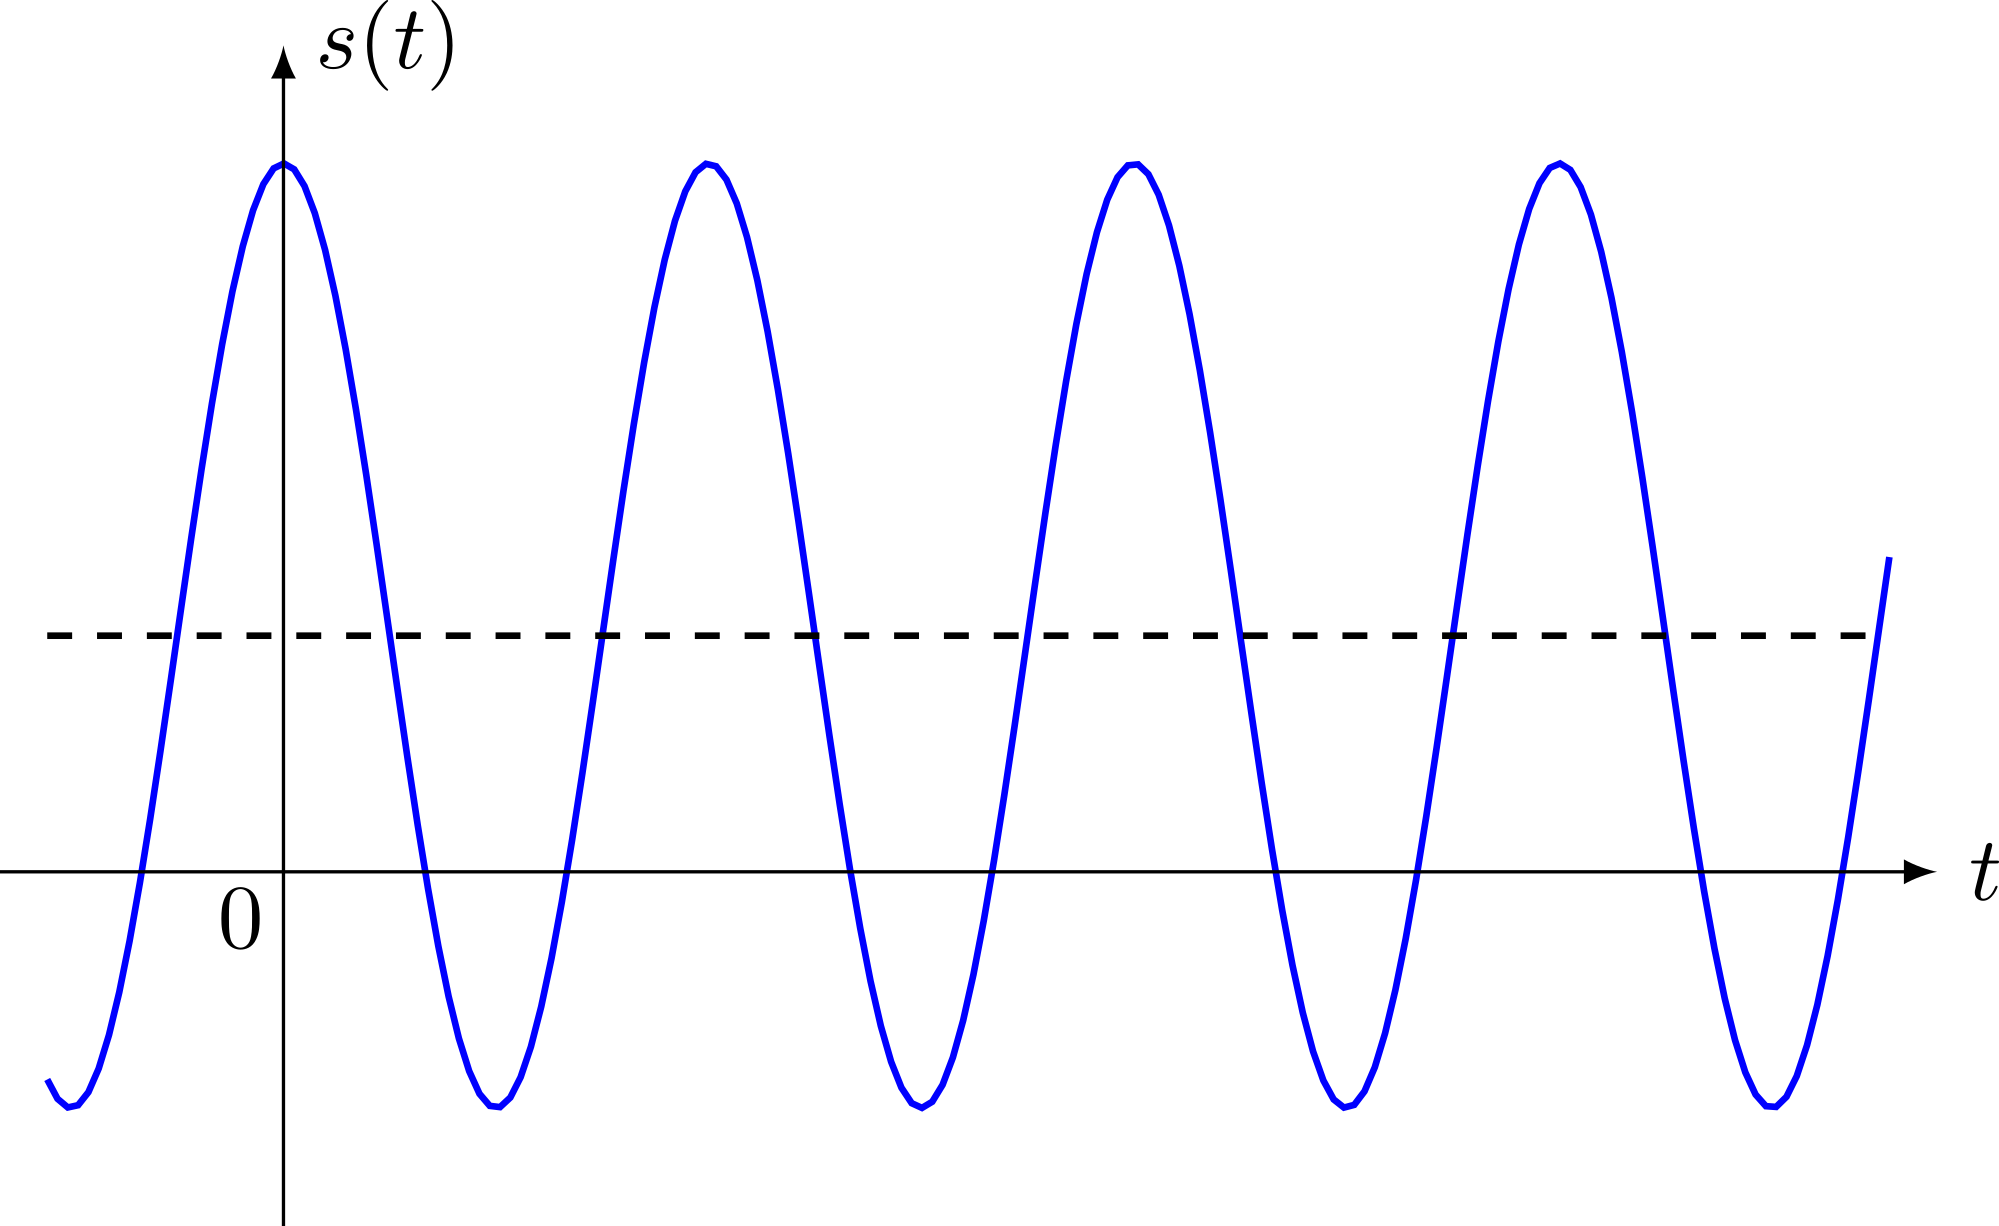
\includegraphics[width=.5\linewidth]{moy_cos-S0}
\end{center}

\subsection{Valeur efficace}
\begin{center}
    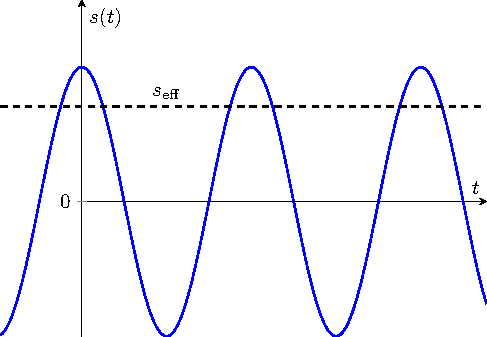
\includegraphics[width=.5\linewidth]{veff_cos}
\end{center}

\section{Décomposition en série de \textsc{Fourier}}

\subsection{Théorème de \textsc{Fourier}}

\subsection{Analyse spectrale}
% Olivier

\subsection{Relation de \textsc{Parseval}}

\section{Filtrage}
\subsection{Traitement du signal et filtre}

\subsection{Fonction de transfert d'un filtre}

\begin{rexem}{Exemple}
    Le filtre RC~!
\end{rexem}

\subsection{Effet d'un filtre sur un signal périodique}

% Olivier + Corot p.19

\section{Description d'un filtre}

\begin{center}
    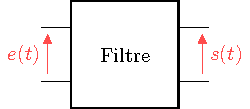
\includegraphics[width=.5\linewidth]{filtre_plain}
\end{center}

\subsection{Gain et gain en décibels}

\subsection{Diagramme de \textsc{Bode}}
\subsubsection{Définition}

\subsubsection{Asymptotes}
% Corot p.7

\subsubsection{Lecture}

\subsection{Filtres moyenneurs, dérivateurs et intégrateurs}
% Corot p.20, Schwei p.7

\section{Exemples de filtres d'ordre 1}
\subsection{RC sur C~: passe-bas}
\subsubsection{Schéma}
\subsubsection{Prévision comportement}
\subsubsection{Fonction de transfert, généralisation}
\subsubsection{Diagramme de \textsc{Bode}}
\begin{center}
    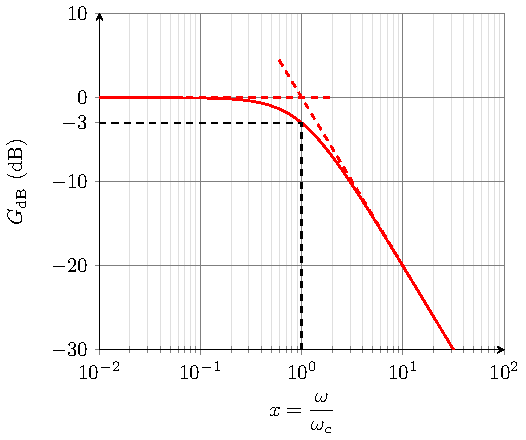
\includegraphics[width=0.48\linewidth]{RCC_bode-gain}
    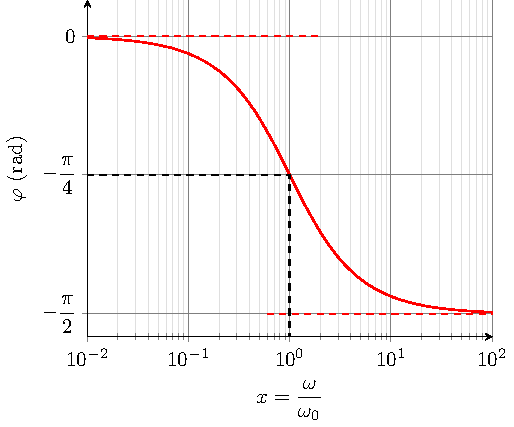
\includegraphics[width=0.48\linewidth]{RCC_bode-phase}
\end{center}
\subsubsection{Comportement dérivateur à BF}

\subsection{RC sur R~: passe-haut}
\subsubsection{Schéma}
\subsubsection{Prévision comportement}
\subsubsection{Fonction de transfert, généralisation}
\subsubsection{Diagramme de \textsc{Bode}}
\begin{center}
    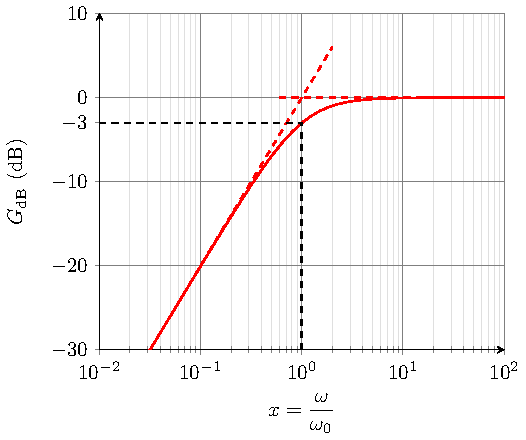
\includegraphics[width=0.48\linewidth]{RCR_bode-gain}
    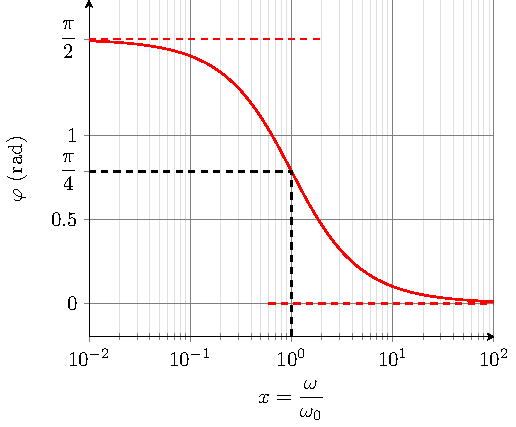
\includegraphics[width=0.48\linewidth]{RCR_bode-phase}
\end{center}
\subsubsection{Comportement intégrateur à HF}

\section{Exemples de filtres d'ordre 2}
\subsection{RLC sur C~: passe-bas ordre 2}
\subsubsection{Schéma}
\subsubsection{Prévision comportement}
\subsubsection{Fonction de transfert, généralisation}
\subsubsection{Diagramme de \textsc{Bode}}
\begin{center}
    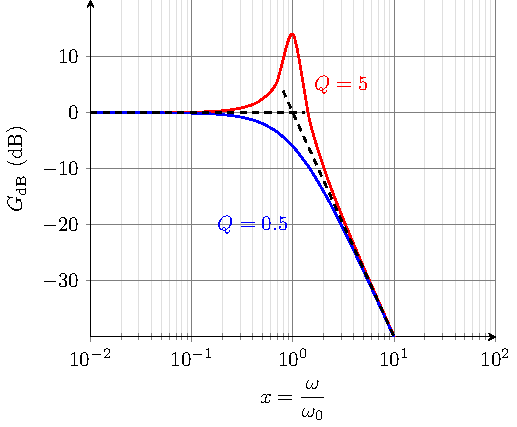
\includegraphics[width=0.48\linewidth]{RLCC_bode-gain}
    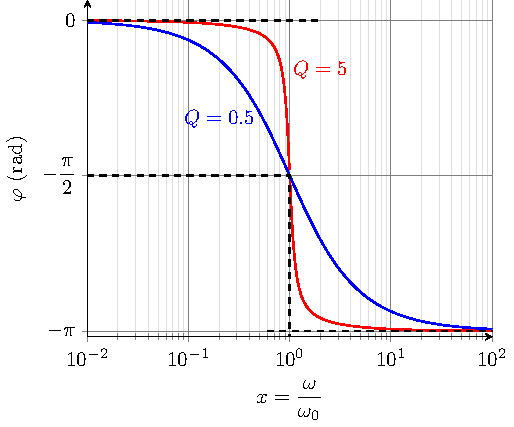
\includegraphics[width=0.48\linewidth]{RLCC_bode-phase}
\end{center}

\subsection{RLC sur R~: passe-bande}
\subsubsection{Schéma}
\subsubsection{Prévision comportement}
\subsubsection{Fonction de transfert, généralisation}
\subsubsection{Diagramme de \textsc{Bode}}
\begin{center}
    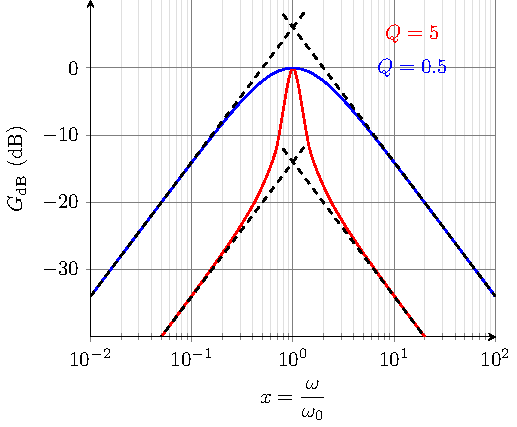
\includegraphics[width=0.48\linewidth]{RLCR_bode-gain}
    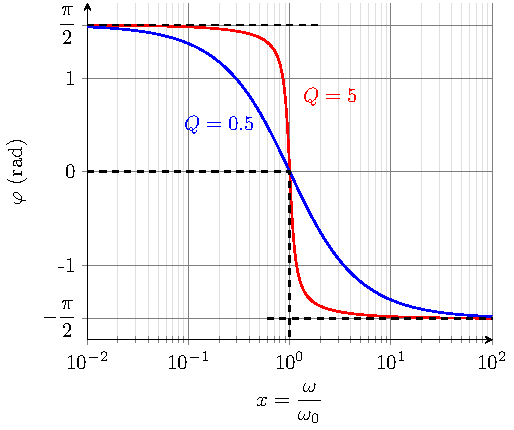
\includegraphics[width=0.48\linewidth]{RLCR_bode-phase}
\end{center}

\section{Résumé}

\section{Filtres en cascade}

\end{document}
